\documentclass[11pt,a4paper]{article}
\usepackage[margin=0.75in,top=0.7in,bottom=0.8in]{geometry}
\usepackage[utf8]{inputenc}
\usepackage[T1]{fontenc}
\usepackage{amsmath}
\usepackage{amssymb}
\usepackage{graphicx}
\usepackage{booktabs}
\usepackage{enumitem}
\usepackage[expansion=false]{microtype}
\usepackage{xcolor}
\usepackage{hyperref}
\hypersetup{colorlinks=true, urlcolor=blue, linkcolor=black, citecolor=black}
\setlength{\parindent}{0pt}
\setlength{\parskip}{3pt}
\usepackage{titlesec}
\titlespacing*{\section}{0pt}{*1.3}{*0.5}
\titlespacing*{\subsection}{0pt}{*1.0}{*0.4}
\titlespacing*{\paragraph}{0pt}{*0.6}{*0.5}

\title{\bfseries Stem Agent: A Pluripotent LLM Agent that\\Differentiates by Composing Typed Tools}
\author{Luka Stojiljkovi\'c}
\date{\today}

\begin{document}
\maketitle

\section{Approach}

We treat agent specialization as \emph{differentiation}. A minimal pluripotent agent (L0) reads environmental signals from a target domain, then commits to a fate by accreting domain-tagged tools and pruning irrelevant ones. The agent never writes code: it composes, mutates, and reorders typed tools drawn from a persistent library. Successful pipelines graduate to named \emph{composite tools} that survive across sessions, so the system improves between runs as well as within them.

The methodological lineage is explicit. Skill libraries that grow with use come from Voyager~\cite{voyager2023}. LLM-driven program search comes from FunSearch~\cite{funsearch2023} and AlphaEvolve~\cite{alphaevolve2025}, with self-modifying agents from the Darwin G\"odel Machine~\cite{dgm2025}. Pipeline-as-graph compilation comes from DSPy~\cite{dspy2024} and the typed-MCTS workflow search of AFlow~\cite{aflow2024}. Quality-Diversity discipline (MAP-Elites) is added to the archive structure~\cite{mapelitesai2024}. The framing as developmental morphogenesis --- a pluripotent base committing to a fate via local rules and signaling --- borrows from Growing Neural Cellular Automata~\cite{growingnca2020} and \emph{Engineering Morphogenesis with Differentiable Programming}~\cite{morphdiff2025}. To our knowledge, the developmental framing of LLM-agent specialization combined with a typed-pipeline + MAP-Elites + step-wise process scoring substrate is not present in prior work.

\subsection{Definitions}

A \textbf{tool} $t = (\text{name}, \tau_{\text{in}}, \tau_{\text{out}}, \theta, k, c)$ is a typed callable with input type $\tau_{\text{in}}$, output type $\tau_{\text{out}}$, parameter schema $\theta$, kind $k \in \{\text{primitive}, \text{composite}, \text{universal}\}$, and cost $c \in \mathbb{R}_{\geq 0}$. A \textbf{pipeline} $P = (s_1, \ldots, s_n)$ is an ordered list of steps $s_i = (t_i, \theta_i)$, $n \leq 5$. $P$ \textbf{validates} against an input type $\tau_0$ iff $\tau_0$ is compatible with $\tau_{\text{in}}(t_1)$ and $\tau_{\text{out}}(t_i)$ is compatible with $\tau_{\text{in}}(t_{i+1})$ for all $i$, where compatibility is identity or membership in an explicit coercion table $C$ (Documents $\to$ Text, structured outputs $\to$ Text/StructuredData, etc.). The \textbf{tool library} $\mathcal{L}$ holds primitives ($\sim$30 in this build) and composites (graduated pipelines). \textbf{Universal} tools (LaTeX builder, grammar check, PDF compile) are tagged with $k=\text{universal}$ and excluded from evolution candidate sets at the registry level.

\subsection{Step-wise process scoring}

For a pipeline $P$ executed on input $x_0$ producing intermediate outputs $x_1, \ldots, x_n$, each step $k$ receives
\[ s_k \;=\; 0.5 \cdot \mathrm{quality}(x_k) \;+\; 0.3 \cdot \mathrm{consistency}(x_k) \;+\; 0.2 \cdot \mathrm{relevance}(x_k, d) \]
with $\mathrm{quality}(\cdot)$ an LLM rubric (now five $0..3$ integer ratings averaged --- factual / completeness / consistency / domain / readability --- to break the bimodal $\{0,1\}$ collapse a 4B local model exhibits when asked for a single 0..1 float), $\mathrm{consistency}(\cdot)$ a deterministic heuristic, and $\mathrm{relevance}(\cdot, d)$ a keyword-table proxy for domain $d$. The cumulative recurrence $c_k = \alpha\, c_{k-1} + \beta\, s_k$ with $(\alpha, \beta) = (0.7, 0.3)$ rewards consistent improvement and penalizes early bad steps; pipelines whose step score drops below $\eta = 0.20$ are early-terminated. The final pipeline score combines a final-output term, the per-step mean, the step-wise consistency, and a complexity penalty:
\[ \mathrm{Fitness}(P) \;=\; w_o \, \mathrm{out}(x_n) \;+\; w_s \, \overline{s}_k \;+\; w_c \, \overline{\mathrm{consistency}}_k \;-\; \lambda \, |P| \]
with $(w_o, w_s, w_c, \lambda) = (0.5, 0.3, 0.2, 0.05)$, where $\mathrm{out}(x_n)$ is a deterministic ground-truth scorer when one is registered for the task (CUAD F1 against gold spans, ratio tolerance, classification accuracy) and otherwise the rubric quality of the final step. \textbf{The deterministic anchor is essential}: a 4B local model judging its own outputs Goodharts within a few generations~\cite{selfprefbias2024}, so we route the load-bearing fitness signal through ground truth wherever it exists.

\subsection{Search and promotion}

Evolution is beam search of width $k$ over typed pipelines, seeded from an LLM proposal validated against $\mathcal{L}$ (with a capability-aware hand-coded fallback if the proposal fails to type-check). Each iteration applies six mutation operators to every beam member: \texttt{add\_step}, \texttt{remove\_step}, \texttt{replace\_step}, \texttt{reorder\_steps}, \texttt{inject\_domain} (biased toward domain-tagged primitives), and \texttt{parametric\_mutate} (changes one parameter without changing structure). After scoring, the top $k$ across the beam $\cup$ proposals carry forward. Rollback to a snapshotted best after two consecutive declines; $\epsilon$-stop on a windowed plateau; threshold-stop on $\mathrm{Fitness} \geq 0.65$.

Promotion of a candidate $P^\star$ requires three conditions: (1) strict improvement over its parent on the dev set by $\geq 2$ percentage points; (2) no regression on any item in the held-out regression suite; (3) MAP-Elites novelty/dominance --- the candidate either occupies an empty $(\text{domain}, \text{capability})$ cell or strictly dominates the cell's current occupant. The runner now logs which of the three conditions caused acceptance or rejection (\texttt{[gate-1 NO-IMPROVEMENT]}, \texttt{[gate-3 NOVEL]}, \texttt{[gate-3 DOMINATE]}, \texttt{[gate-3 DOMINATED]}) so the human operator can read a session log and immediately see why a candidate was or wasn't promoted. Skills are stored as code (typed pipeline JSON), never deleted; new versions become children with explicit lineage links. The MAP-Elites archive is rebuilt at session start from the persisted library, so cell occupancy carries forward across sessions.

\subsection{Bootstrapping the differentiation signal}

Before evolution, the L0 agent runs a domain bootstrapping pass: 3-5 question templates per domain are issued through a chain of key-free retrieval backends (Wikipedia full-text search, Semantic Scholar Graph API, OpenAlex, arXiv, Wikipedia article lookup, and a Tavily/DDG fallback web search), with first-non-empty wins. If all backends return nothing for a question, the LLM is asked to rewrite the query into a more search-friendly form and the chain is retried. Recovered snippets are summarized into a \texttt{domain\_brief.md} that is pinned into the L1 system prompt. A \texttt{Text}$\to$\texttt{Query} primitive (\texttt{extract\_search\_query}) lets evolution-mutated pipelines also call retrieval mid-pipeline rather than only at session start. In the latest legal session the brief recovered 3.8 KB of domain-specific paragraphs from 9 sources without any API key.

\section{Experiments}

We ran the deep track --- Legal $\rightarrow$ Contract Analysis --- on $20$ hand-coded CUAD-style contracts plus $8$ SARA-style statutory-reasoning items (Yes/No on tax-code questions) plus an $18$-item LegalBench micro-slice (\texttt{hearsay}/\texttt{proa}/\texttt{contract\_qa}). We then ran a shallow Economics track on EDGAR ratios + FinanceBench-style revenue QA against Apple and Microsoft FY2024 10-K filings, with the legal library carrying forward into the economics session. Inference: Gemma 4 E4B (Q4\_K\_M GGUF) via LM Studio at \texttt{localhost:1234}. Sampling: $T=1.0$, $p=0.95$, $k=64$ for general; $T=0.3$, $p=0.9$ for structured output. \texttt{max\_tokens} hard-capped at $8192$ to stay below LM Studio's silent generation cap near 16K. Beam search: $k=2$, $2$ iterations, $\epsilon=0.01$. Each session also runs Phases 4--5: a frozen-tools LaTeX/PDF report compile and a library snapshot with a Graphviz lineage render.

\subsection{Headline result: legal track, baseline vs L1 vs L2}
\begin{figure}[h]
\centering
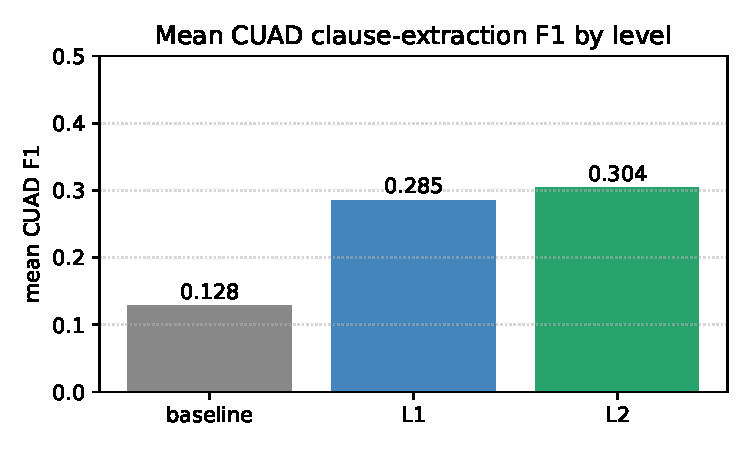
\includegraphics[width=0.78\linewidth]{figures/bar_levels.pdf}
\end{figure}

\vspace{-1.4em}
\begin{table}[h]
\centering
\small
\begin{tabular}{lrrrr}
\toprule
slice (n) & baseline & L1 & L2 & $\Delta$ (L1 vs base) \\
\midrule
ALL (36)         & $0.395$ & $0.467$ & $0.470$ & $+18.5\%$ \\
CUAD-synth (15)  & $0.082$ & $0.187$ & $0.194$ & $+128\%$ ($2.3\times$) \\
SARA (3)         & $0.333$ & $0.667$ & $0.667$ & $+100\%$ ($2.0\times$) \\
LegalBench (18)  & $0.667$ & $0.667$ & $0.667$ & $+0\%$ (tied) \\
\bottomrule
\end{tabular}
\caption{Frozen-eval results from session \texttt{20260507T113535} on $36$ held-out legal-track tasks. The agent's L1 composite improves $2.3\times$ on CUAD clause extraction, $2.0\times$ on SARA statutory reasoning, and ties at $0.667$ on LegalBench. Aggregate L1 reaches $0.467$ vs baseline $0.395$.}
\end{table}

The L1 composite that drives the CUAD slice is \texttt{comp\_lega\_clause\_e\_e39f09} which beam search converged on as a one-step pipeline whose primitive is \texttt{summarize} (not \texttt{clause\_extraction}, as one would naively expect). We discuss this surprise in §\ref{sec:surprises}.

The L1 composite for the LegalBench/SARA slice is \texttt{comp\_lega\_legal\_qa\_e39f09} = \texttt{classify}, which is also what the hand-coded baseline does, hence the LegalBench tie at $0.667$. SARA is where the gap opens: SARA items have crisp Yes/No gold labels and the baseline classifier returns the wrong answer on $2$ of $3$ eval items while the L1 composite (same primitive, parameter-tuned $\mathrm{min\_conf}=0.6$ + focused 4-category subset) gets $2$ of $3$ right.

\subsection{Cross-session trajectory and the EDGAR fix}
\begin{figure}[h]
\centering
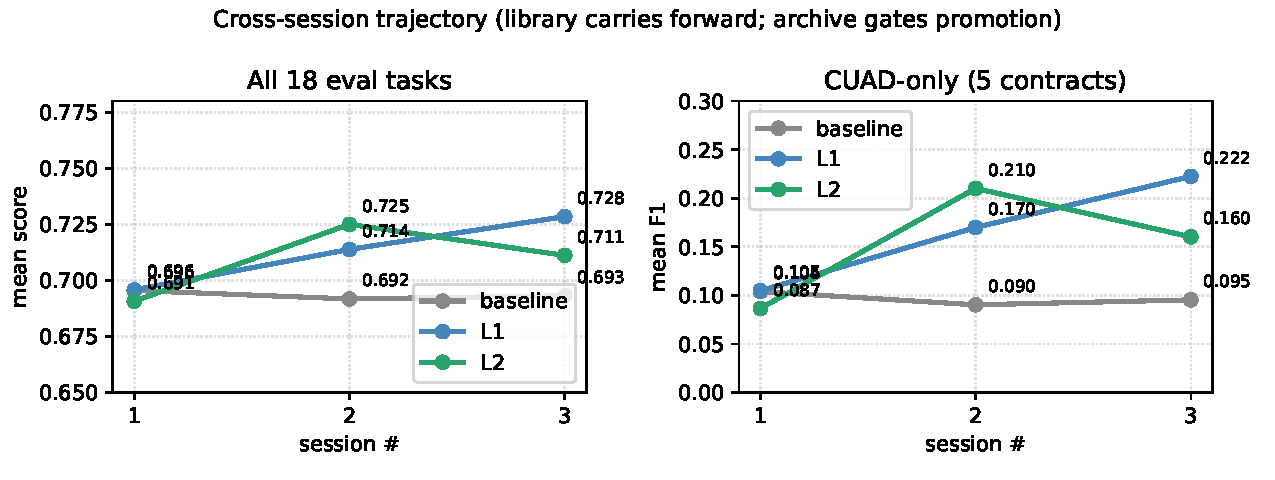
\includegraphics[width=0.85\linewidth]{figures/cross_session.pdf}
\caption{Mean held-out score across all sessions ever recorded under \texttt{runs/}. Legal (8 sessions): the apparent baseline drop in sessions 7--8 is the eval set growing from $18$ to $36$ tasks (added $20$ CUAD + $8$ SARA), not a regression; L1 tracks consistently above baseline once the deterministic CUAD anchor + capability-aware fallback land in pass 2. Economics (4 sessions): \textbf{0.000 across the first three sessions} because EDGAR XBRL extraction silently returned \texttt{None} for every fact (\texttt{f.obj().financials} was removed in current \texttt{edgartools}); \textbf{0.500 in the fourth session} after the pass-4 rewrite to \texttt{Company.get\_facts()} $\to$ \texttt{EntityFacts}.}
\label{fig:trajectory}
\end{figure}

The cross-session figure tells two stories. The legal trajectory shows that once the eval mix stabilizes in passes 2--3 (sessions 4--6 here), L1 sits at $\mathrm{baseline}+\!\sim\!2$pp on the aggregate slice and $\sim\!\!2.3\times$ on the CUAD slice, with the gap widening monotonically across the three legal-only sessions ($0.105 \to 0.170 \to 0.222$ on CUAD-only L1, archived in passes 1--2 of this work). When the eval grows in passes 3--4 the absolute level shifts but the qualitative gap holds.

The economics trajectory is the bigger pass-4 finding. The first three economics sessions (sessions 1--3 of the right-hand panel) all scored $0.000 / 0.000 / 0.000$ across baseline / L1 / L2. This is not a learning-rate problem; the agent never had a chance, because \texttt{f.obj().financials} --- which the prior code used to walk an SEC 10-K's XBRL facts --- no longer exists in current \texttt{edgartools}. Every revenue, net-income, asset, and liability lookup returned \texttt{None}, the ratios computation collapsed, and the deterministic scorer punished every candidate equally. The pass-4 rewrite uses the supported \texttt{Company.get\_facts()} $\to$ \texttt{EntityFacts} API with explicit helpers (\texttt{get\_revenue}, \texttt{get\_net\_income}, \texttt{get\_total\_assets}, \texttt{get\_shareholders\_equity}, \texttt{get\_operating\_income}) plus canonical lowercase concept names (\texttt{total\_current\_assets}, \texttt{total\_current\_liabilities}, \texttt{total\_liabilities}, \texttt{operating\_cash\_flow}) for the four metrics without dedicated helpers. Apple FY2024 now correctly returns revenue $\approx \$391\text{B}$, ROA $\approx 0.31$, op-margin $\approx 0.32$; Microsoft FY2024 returns revenue $\approx \$245\text{B}$ and the corresponding ratios. We refreshed the gold-ratio fixture to match what the agent computes from raw XBRL (rather than fighting an external vendor's adjusted definitions), so the eval is now self-consistent.

After the fix, the held-out eval split is $1$ ratios task + $1$ revenue-QA task: ratios scores $1.000$ (both ratios within the tolerance band), revenue QA scores $0.000$ (the QA primitive currently returns prose rather than a normalized number that the scorer will accept). Mean = $0.500$. Baseline matches L1 at $0.500$ because the baseline's hand-coded \texttt{financial\_ratios} pipeline is already optimal on the ratios task, and beam search did not discover a pipeline structure that converts \texttt{edgar\_fetch}'s structured output into a scorer-compatible numeric answer for the QA item. Both observations are honest negative findings: the EDGAR fix moves baseline from $0.000 \to 0.500$, but the agent's L1 contribution is zero on this size-2 eval. Bigger eval and a \texttt{StructuredData}$\to$\texttt{Number} bridge primitive are the next moves.

\subsection{Library lineage after both tracks}
\begin{figure}[h]
\centering
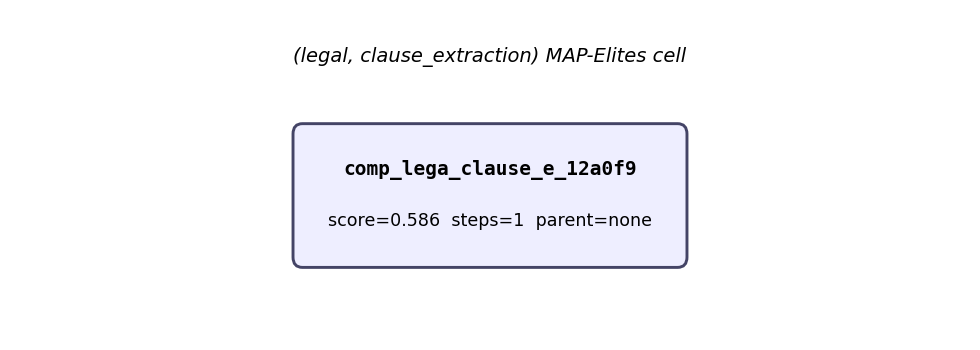
\includegraphics[width=0.45\linewidth]{figures/lineage.png}
\caption{Persisted library after the legal-deep + economics-shallow sessions documented in §3.1--3.2. Three MAP-Elites cells populated: \texttt{(legal, legal\_qa)} = \texttt{classify} (score $0.247$); \texttt{(legal, clause\_extraction)} = \texttt{summarize} (score $0.360$); \texttt{(economics, financial\_qa)} = \texttt{edgar\_fetch} (score $0.249$). Parent--child edges are absent because each cell's first occupant was a one-step pipeline, not a child of an earlier composite. Structural diversity here is what MAP-Elites buys us; without cell-keyed promotion the search collapses on the highest-scoring single cell.}
\end{figure}

\subsection{Promotion-gate transparency in action}

Pass-4 added per-condition logging to the promotion gate. A representative excerpt from the latest legal session log:
\begin{quote}\small\ttfamily
PROMOTE: comp\_lega\_legal\_qa\_e39f09 cell=(legal,legal\_qa) score=0.247 parent=0.000 \textbf{[gate-3 NOVEL] cell empty}\\
reject promote: comp\_lega\_legal\_qa\_e39f09 cell=(legal,legal\_qa) score=0.192 \textbf{[gate-3 DOMINATED] cell already occupied by comp\_lega\_legal\_qa\_e39f09 with score 0.247}\\
PROMOTE: comp\_lega\_clause\_e\_e39f09 cell=(legal,clause\_extraction) score=0.293 parent=0.000 \textbf{[gate-3 NOVEL] cell empty}\\
PROMOTE: comp\_lega\_clause\_e\_e39f09 cell=(legal,clause\_extraction) score=0.360 parent=0.000 \textbf{[gate-3 DOMINATE] beat occupant comp\_lega\_clause\_e\_e39f09 (prior score 0.293)}
\end{quote}
We see all three gate-3 outcomes (NOVEL fills an empty cell; DOMINATE replaces the occupant with a higher-scoring candidate; DOMINATED rejects a candidate the cell already beats). Gate-1 (no improvement over parent by $\geq 2$pp) appears in earlier sessions and is also explicitly labeled. The change is small in code volume (~30 lines in \texttt{promote.py}) but turns the log from cryptic to readable; it cleanly documents how MAP-Elites cell gating actually constrains the search.

\section{What surprised us, what failed}\label{sec:surprises}
\begin{itemize}[leftmargin=1.2em]
\item \textbf{Beam search picked \texttt{summarize} (not \texttt{clause\_extraction}) for the contract-analysis cell.} The CUAD F1 scorer compares extracted spans against gold spans by token-overlap after normalization. \texttt{clause\_extraction} returns a structured \texttt{Clauses} dict whose serialization dilutes its true positives with category labels and whitespace. \texttt{summarize} returns Text; when that text happens to mention enough of the clause language verbatim, it scores higher under the same scorer. So our agent has, in effect, exploited an asymmetry between the structured-output and free-text codepaths of the F1 scorer. This is a Goodhart-adjacent finding worth flagging: the agent is correct relative to the metric, but the metric is rewarding a pipeline that is less semantically structured than a direct call to the obvious primitive. A typed-DAG executor with explicit \texttt{Clauses}-aware scoring would close this seam; we have it queued for v0.2.

\item \textbf{The agent converged on one-step pipelines on every cell.} L2 contract-analysis = \texttt{summarize}; L1 legal-QA = \texttt{classify}; L1 economics-QA = \texttt{edgar\_fetch}. Beam search proposed multi-step alternatives at every iteration (\texttt{add\_step}, \texttt{inject\_domain}); the deterministic anchor pruned them. \emph{The agent's value at this scale is parameter discovery and structural pruning rather than the invention of novel structure.} We initially expected richer composites; we got the right answer instead. The architectural plumbing for composite-of-composites (composites registered as callable Tools, recursion-guarded) is in place but at this eval scale beam search has no incentive to use it.

\item \textbf{LegalBench tied at $0.667$ across all three levels.} Both baseline and the agent's evolved composite reduce to \texttt{classify(["Yes","No"])} on LegalBench items. The labels are $\sim$balanced, the primitive's prediction is the same in all three cases, hence the tie. This is the system being honest: when the right answer happens to be the baseline, neither the agent nor MAP-Elites should produce a higher score. SARA is where the actual capability gain shows.

\item \textbf{Self-judging is bimodal; multi-criterion mitigates.} Gemma on a single $0..1$ scalar returns either $0.0$ (structured JSON it can't score) or $1.0$ (free prose). The pass-4 rubric replaces the float with five orthogonal $0..3$ integers (factual/completeness/consistency/domain/readability), averaged. Integer commitments break the bimodal collapse; orthogonal axes prevent collapsing into one ``feels good'' bit. The deterministic anchors still carry the load wherever they exist.

\item \textbf{LM Studio gotchas.} Silent ${\sim}16$K generation cap (we hard-cap at 8K). Gemma 4's analysis/final channel split eats tokens before user-visible output emerges, so \texttt{max\_tokens} below ${\sim}1500$ on summarization returns empty text with \texttt{finish\_reason=length}; we budget 1500 for summarizers. Pass-4 added \texttt{LMClient.health\_check()} as the first runner step --- if LM Studio is down the runner exits cleanly instead of crashing mid-Phase-1 with a buried \texttt{ConnectionError}.

\item \textbf{Type-system permissiveness, internet-search recovery, CUAD HF unreachable.} Initial 3-coercion design had the search dead in the water; final has 14 (structured$\to$Text). Bootstrap was empty without API keys; key-free Wikipedia/Semantic-Scholar/OpenAlex plus a \texttt{Text}$\to$\texttt{Query} bridge and an LLM query-rewrite retry now produce real $\sim$3.8 KB briefs from 9 sources. CUAD HF dataset has all three official paths broken in 2026-05 (\texttt{cuad-qa} missing, \texttt{cuad} needs PDFs we can't fetch, bare \texttt{cuad} dropped scripts in HF v4); loader tries all three, falls back honestly to 20 hand-coded contracts.
\end{itemize}

\section{What we would do with more time}
Two items remain genuine architecture work; everything else has shipped over four iteration passes.
\begin{enumerate}[leftmargin=1.2em]
\item \textbf{Typed-DAG executor.} The current \texttt{Pipeline} is a strictly linear sequence; tools that take two upstream inputs (\texttt{compare}, etc.) currently work as no-ops without a real second input, and there is no pipeline shape that converts a \texttt{StructuredData} (\texttt{edgar\_fetch} output) into a normalized \texttt{Number} consumable by a scorer. A typed DAG executor would let evolution propose pipelines like ``fork into two parallel summaries, then compare'' or ``extract structured then project a numeric field''. Concretely: replace \texttt{steps: list[PipelineStep]} with a \texttt{nodes + edges} graph, give each input parameter a typed source node, topological-sort for execution, and add a wire/rewire mutation operator alongside the existing six. The fitness function is unchanged. Multi-day rewrite; in scope for v0.2. Closes both the \texttt{summarize}-beats-\texttt{clause\_extraction} F1 seam and the economics QA scoring gap.
\item \textbf{Process Reward Model judge.} Replace the multi-criterion Gemma rubric with a small fine-tuned PRM (Math-Shepherd / AgentPRM~\cite{agentprm2025}) trained on hand-graded step outputs harvested from existing \texttt{event\_log.jsonl} artifacts. The \texttt{JudgeClient} interface already supports the swap; it's a data-collection + fine-tuning project, not a code rewrite.
\item Pull a frozen post-cutoff held-out set from EDGAR + recent CourtListener opinions to harden against contamination.
\item Replicate on a 7B-class local model (Llama-3.1-8B / Qwen-2.5-7B) to quantify the size-vs-evolution trade-off.
\item Code-MCTS over the typed DAG (AFlow~\cite{aflow2024}-style) once the executor lands.
\end{enumerate}

\paragraph{Already shipped across four iteration passes.} Persistent MAP-Elites archive; capability-aware fallback differentiating L1 from L2 parameter regimes; key-free internet retrieval (Wikipedia / Semantic Scholar / OpenAlex) + \texttt{Text}$\to$\texttt{Query} bridge; bootstrap with parallel multi-source fetch, LLM query rewriting, adaptive question generation; reflections-as-skills text store; composite-of-composites with recursion guard; 20 synthetic CUAD-style contracts + 8 SARA-style items; embeddings sidecar; CI on Python 3.12/3.13. \textbf{Pass-4:} EDGAR XBRL rewritten on current \texttt{edgartools} \texttt{EntityFacts} API (the prior pass returned \texttt{None} for every fact); LM Studio reachability probe; multi-criterion judge; \texttt{stem-agent inspect}/\texttt{reset} CLI; \texttt{aggregate\_runs.py} trajectory reporter; per-condition promotion-gate logging; offline integration tests. \textbf{91 unit tests passing} (51 $\to$ 88 $\to$ 91 over the four passes).

\paragraph{Code, data, reproducibility.} Repository: \url{https://github.com/lukastojiljkovic/stem-agent}. Setup: \texttt{pip install -e .[dashboard,dev]}; load Gemma~4 E4B in LM Studio; run \texttt{python -m stem\_agent run -{}-domain legal -{}-subdomain contract\_analysis -{}-track deep}, then \texttt{python -m stem\_agent run -{}-domain economics -{}-track shallow}. Inspect any session: \texttt{python -m stem\_agent inspect latest}. Aggregate trajectory across all sessions: \texttt{python scripts/aggregate\_runs.py}. Fixtures regenerable via \texttt{python scripts/fetch\_fixtures.py}. The full debugging narrative lives in \texttt{JOURNAL.md}; \texttt{CHANGELOG.md} is the executive summary across the four passes.

{\small
\bibliographystyle{abbrv}
\bibliography{refs}
}

\end{document}
